\begin{figure*}[tbp]
  \centering
  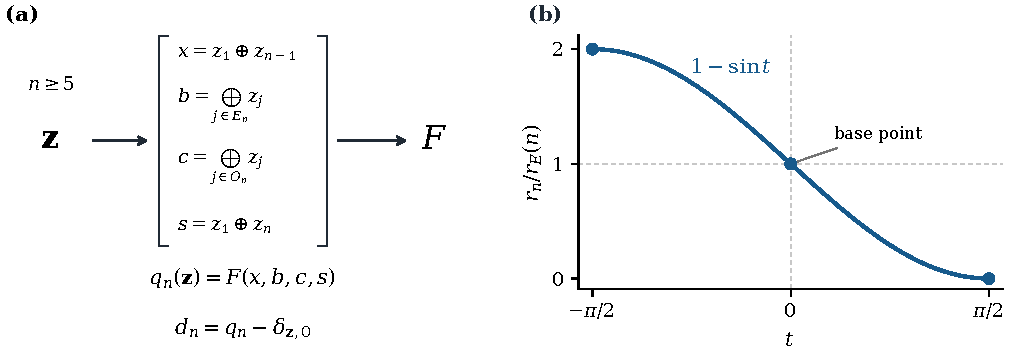
\includegraphics[width=\textwidth]{figures/fig1_unified.pdf}
  \caption{Unified phase deformation for every $n\geq5$.
  (a) Four linear Boolean features feed the same kernel $F$; the only removed support point is the physical string $\mathbf z=0$.
  The blocks $E_n$ and $O_n$ contain the even and odd indices in $[2,n-2]$, respectively.
  (b) The normalized common Bloch radius $r_n(t)/r_E(n)=1-\sin t$ on $[-\pi/2,\pi/2]$, where $r_E(n)=\sqrt3/2^{n-1}$ is the reference radius.
  From left to right, the marked points give the enhanced endpoint, the specified EJM at $t=0$, and the endpoint with maximally mixed one-qubit marginals.}
  \label{fig:unified}
\end{figure*}
